\title{ Weld pool detection and geometrical analysis during GTAW process by image processing library}


\section{Introduction}

Gas Tungsten Arc Welding (GTAW), which uses a non-consumable tungsten 
electrode and an inert gas for arc shielding, is an extremely 
important arc welding process. It is commonly used for welding hard-to-weld
 metals such as stainless steel \cite{JUANG} and therefore widely use in 
modern and basic industries. To achieve good weld quality in GTAW process,
 several weldment characteristics or objects should be sensed and
 controlled \cite{DOUMANIDIS}. It is shown that the geometry of the weld 
pool, in particular his shape and size, contains sufficient information
 about weld penetration to evaluate the weld quality \cite{ZHANG}.
 Furthermore it has been shown that the welding arc parameters to 
simulation and weld quality are directly relate to the weld pool 
geometry \cite{LU}.
Basically the weld pool object is the key in quality control 
to automated welding process \cite{KOVACEVIC}. 
According to this a better comprehension of weld pool behavior
 presents a GTAW process, could help to improve numerical 
simulations and enhance welding quality in manufacturing 
process \cite{LIN}, \cite{WU1}. 

There have been many studies on visual sensing techniques
 for observing weld pool image \cite{BAE}. Optical sensors
 like high speed CCD cameras and lighting systems have been
 widely use in GTAW process to realize image acquisition 
\cite{GUANGJUN}, control process \cite{BAE} and parametric 
studies \cite{BALSAMO}. Then image processing plays a critical
 role in extracting useful information from visual scenes 
\cite{WANG}. Nevertheless the strong interference from the
 arc lightning required more than standard image treatment
 to analyses the raw images of the welding process 
\cite{NORDBRUCH}. Previous work has shown that is possible
 to perform geometrical analysis in weld pools \cite{WU1}.
 Parameters such as weld pool contour and surface has been
 detected and measure using different and specifics processing 
images algorithms \cite{KOVACEVIC}, \cite{WU1}, \cite{SAEED}.
 However, to date, effectively automatic images processing 
of GTAW process has not been developed, possibly due to the
 level difficulty involved for welding researchers \cite{WANG}.

To perform geometrical analysis in weld pool; a multipurpose
 C++ based library (erCv) was developed by the Weld/Assembly
 group of LMGC laboratory. These library results from
 selected functions join from highly reliable open source
 libraries to images treatment, geometrical analysis, 
graph theory applications and image visualization.

In a first step, and despite the different static and dynamic 
weld conditions, as well as different current regime, a 
reliable 2D profiles and geometrical parameters from weld
 pool, has been obtained using the mentioned library. 
Using this, a dimension and dimensionless analysis has 
been performed into a static and dynamic GTAW process. 
The intention is contribute to simplify futures numerical
 models of weld pool-arc interaction and quality process.



\section{Problems description}
\label{problem_description}

Indirectly, the weld pool geometry could be detected 
by different methods such pool oscillations \cite{RENWICK}, 
ultrasonic sensing \cite{CARLSON}, radiography \cite{ROKHLIN}.
 However to obtain more precise measurements, direct 
acquisition methods, as vision based techniques, should 
be use \cite{KOVACEVIC}.     Bradstreet was the first 
researcher to experimentally study the bead hump formation
 \cite{CHO}. Humping was defined as the series of 
undulations of the weld bead. Further studies as computer
 simulation made by CHO et al. \cite{CHO} shown a relation
 between the droplet momentum deposition and the hump size.
 Same relations has been found between metal transfer process
 and welding quality \cite{}

Then the shape and size kinetic analysis of macro drop and 
droplets could help to better understand and enhance the PGMAW 
process. To monitoring the shape and size of these welding 
objects, to a first step, a 2D approach would be sufficient.
 Therefore a shadowgraphy technique, or back lighting, is 
the natural choice to record the droplets and macro drops 
profiles \cite{BALSAMO}, furthermore is one of the only way
 to access these quantities. Due to the arc light interference
 and the relatively high speed of wire feed process, a high
 speed camera and an effective image processing algorithms 
are required \cite{WANG}. The typically frame rate acquisition
 to metal transfer drop kinetic analysis is $3000$ per second 
\cite{WANG}. Therefore the algorithms have to be able to extract
 the geometrical information (area, size and others) from 
the macro drop and droplets, from a huge amount of data. 
In addition, the voltage and current signals are directly
 related with the droplet formation at the wire \cite{BALSAMO}.
 Good synchronizations methods have to be applied between 
shadowgraphies frames and electrical signals.



\section{Image processing background}
\label{image_processing_background}

Some definitions and brief description of generals principles used in image processing are required to better understand how is work the algorithms utilized by the erCv library.

\subsection{Some definitions}
\label{some_definitions}

A numerical grey image can be describe as 3D surface discretized by a grid 
mesh in the X,Y plane. Each mesh represents a pixel and the relief surface
 at Z axis, the grey level.  

A strong relief change or high gradient greyness values at the image are
 perceive by human eyes as light changes, and can be interpreted as 
objects edges. 
Sometimes, a regular relief patrons or regular greyness variation 
can be distinguish. The human eyes can perceive these patrons as 
texture and interpret the space between different textures zones as edges.
There exist a large spectrum of algorithms to image treatment, 
in particular to edges detect. Most of them can be classified 
by the way that his operate above the image pixels and grey level.


\subsection{Filters}
\label{filters}

The filters are algorithms that operate as mathematical functions 
$f$ above the $X$, $Y$ or both axis of the image ($Z = f(X,Y)$,  
$f(X)$ or $f(Y)$)  modifying his greyness value or $Z$ component. 
Different kind of filters can be mentioned as median, Gaussian, 
impulse, adaptive and others. The impulse filters such Canny are
 widely use to edge detection \cite{COCQUEREZ}. These filter have
 an impulse response to most important greyness gradient in the 
image; this allows the filter a better edges localisation (see 
figure \ref{photo-explication-filter}). For this reason, Canny 
filter is widely use at erCv library to detect the welding 
elements edges. However, it is sensible to noise or secondary
 greyness gradients in the image and, in consequence, it have 
some difficulties to define closer surface.

\subsection{Snake and level set}
\label{snake-and-level-set}
 
Curve propagation is a popular technique in image analysis 
for object extraction, object tracking, edge detection and 
others (see figure \ref{photo-explication-snake}). The central
 idea behind such an approach is to evolve a curve towards 
the lowest potential of a cost function. However at each 
stage of curve evolution, each curve point potential has 
to be computed. A lot of point (better curve resolution) 
take a lot computing time, and therefore are not yet apply
 to real time detection or relatively speed automatic image
 processing. For this reason snake algorithms are not used at erCv.

\begin{Segmentation}
\label{segmentation}

Let $B$ an image and let $R_{i}$ a region of $B$ such:

\begin{equation}
B = \bigcup_{i}R_{i}\  
\forall i  R_{i} \neq \emptyset\ 
\forall i, j avec i \neq j\ R_{i}\bigcap R_{j} = \emptyset 
\label{equation-segmentation}
\end{equation}

A $B$ segmentation is an image treatment which generate a $B$ 
partition in $R_{i}$ regions. Each region is a connected set of
 pixels with common properties (intensity, texture,...) 
\cite{COCQUEREZ}. The partition is generated by operations
 or comparisons methods between regions. Generally, this 
treatment offers a good detection edges if the elements 
and surrounding area have different textures (see figure
 \ref{photo-explication-segmentation}). 
Note that different regions can belong to the same partition
 and not be placed together, therefore the surface is not 
always connected and, in consequence, the edges of the interest
 regions are not always closed.

\begin{figure}[h!]
\begin{center}    
\subfigure[Weld pool image in static GTAW process]{\label{photo-explication-patron}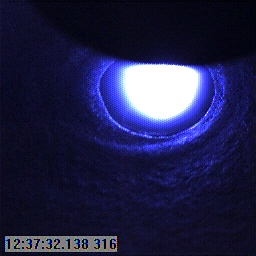
\includegraphics[width=3.5cm,height=3.5cm]{photo-explication-patron.png}}
\subfigure[Canny filter treatment]{\label{photo-explication-filters}\includegraphics[width=3.5cm,height=3.5cm]{photo-explication-filters.png}}\\
\subfigure[Snake treatment]{\label{photo-explication-snake}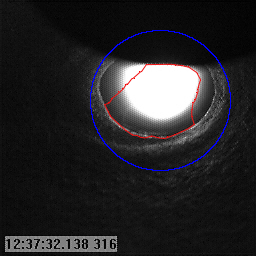
\includegraphics[width=3.5cm,height=3.5cm]{photo-explication-snake.png}}
\subfigure[Segmentation image by 2 cluster sample comparison]{\label{photo-explication-segmentation}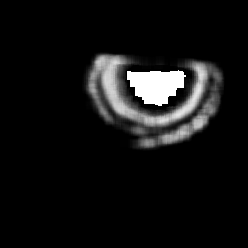
\includegraphics[width=3.5cm,height=3.5cm]{photo-explication-segmentation.png}}
\end{center}
\caption{{\small Samples of different methods technique for image processing}}
\label{photo-explication}
\end{figure}


\section{Image treatment library (erCv)}
\label{image-treatment-library-ercv}

As mentioned, a multipurpose image processing library was developed
 and currently use at the laboratory, in order to analyze welding
 process objects.
erCv is able to perform edge detection and geometrical analysis
 in a different welding objects such: Macro drop, droplets 
(for GMAW process) and weld pool (for GTAW process).
erCv is a modular library assembled in a oriented object C++ 
language. Then erCv is a scalable and portable library able 
to perform real time contour detection. erCv is build in Phyton 
scripts link to C++, making it relatively convivial to use.
erCv is compose by four processing modules based in C,  
C++ and python language (see figure \ref{schema-erCv}). These modules are: 
\begin{description}
\item[Image Treatment:] Due to weld process conditions such
 arc lightening, heat and electrodes positions; the raw image
 registered by CCD camera are not calibrated and present light
 inhomogeneities and noise. In order to obtain the real shape
 and size of weld elements, this module include calibrations
 algorithms. To detect the welding objects contours it is necessary
 to improve the weld element image. This module has the pre-processing
 treatments to noise reduction and image enhancement. Then to start
 the edges detection process, this module includes processing 
algorithms as segmentations by samples comparators, watershed
 transformation, filters edge detectors and histogram based
 methods.  
\item[Geometrical Treatment and Analysis:] This module has 
to end the edge detection process, completing and in some 
cases extrapolating the weld elements edge. It is also 
responsible to compute the geometrical data of welding 
elements such weld pool surface and metal transfer drop 
volumes. This module uses a full geometry algorithm library,
 which include different algorithms such as triangulations 
and mesh generation, alpha shape and convex hull generation
 and polygonal structures.
\item[Graph Theories:] To compute the geometrical data of
 welding elements it is necessary to extract the welding 
object edge from the image; this required some criteria 
such as continuity, length or closer condition.  This module 
use graph algorithms to convert edges pixels points into 
connected segments, and therefore, identify and select the 
welding element edge using the criteria. This module is compose
 by connect segments, estimates minimal cut, determine largest
 chain segments and others algorithms. 
\item[Visualization:] This module is a set of functions use
 to execute, show and/or register the different steps at the
 image process.
\end{description}

\begin{figure}
\begin{center}
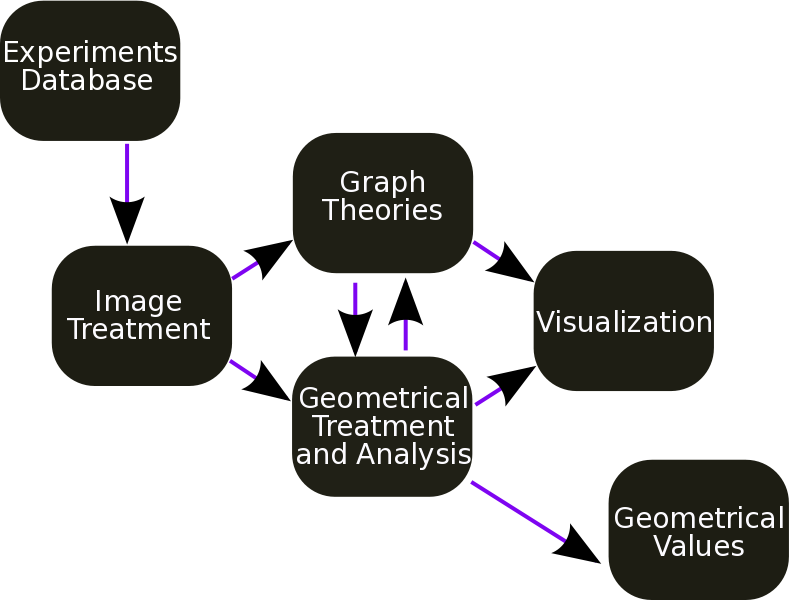
\includegraphics[width=7cm,height=4cm]{schema-erCv.png}
\caption{{\small Flow diagram of erCv library composition}}
\label{schema-erCv}
\end{center}
\end{figure}



\section{Experimental Setup}
\label{experimental_setup}

\subsection{Multi-physics platform}
\label{multi_physics_platform}

The objective is to perform geometrical analysis of weld pool
 in a GTAW process. Notes that geometrical analysis refers to
 surface value and contour detection of weld pool in static and 
dynamic GTAW process. The methods choose is the image treatment 
of recorded image of GTAW static and dynamic process by a high
 speed CCD camera.

To perform the geometrical analyses, different signals have to be 
synchronizes and recorder \cite{CHAPUIS}; therefore an accurate,
 reliable and synchronizes systems are requires due to the high
 amount of data and highly noisy environment (electromagnetic 
noise and arc light radiation). 

A platform has been developed at the laboratory to perform multi-physics
 measures in arc welding process (see figure \ref{schema-platform}). 
The platform was conceive with an automatically procedure to synchronize,
 to acquire, to manage and to exploit large flow of multi-physical
 experimental data (up to 2 Go per test). This characteristic allows
 synchronizing (in time) the current and voltage signals with 
the acquired images.

\begin{figure}
\begin{center}
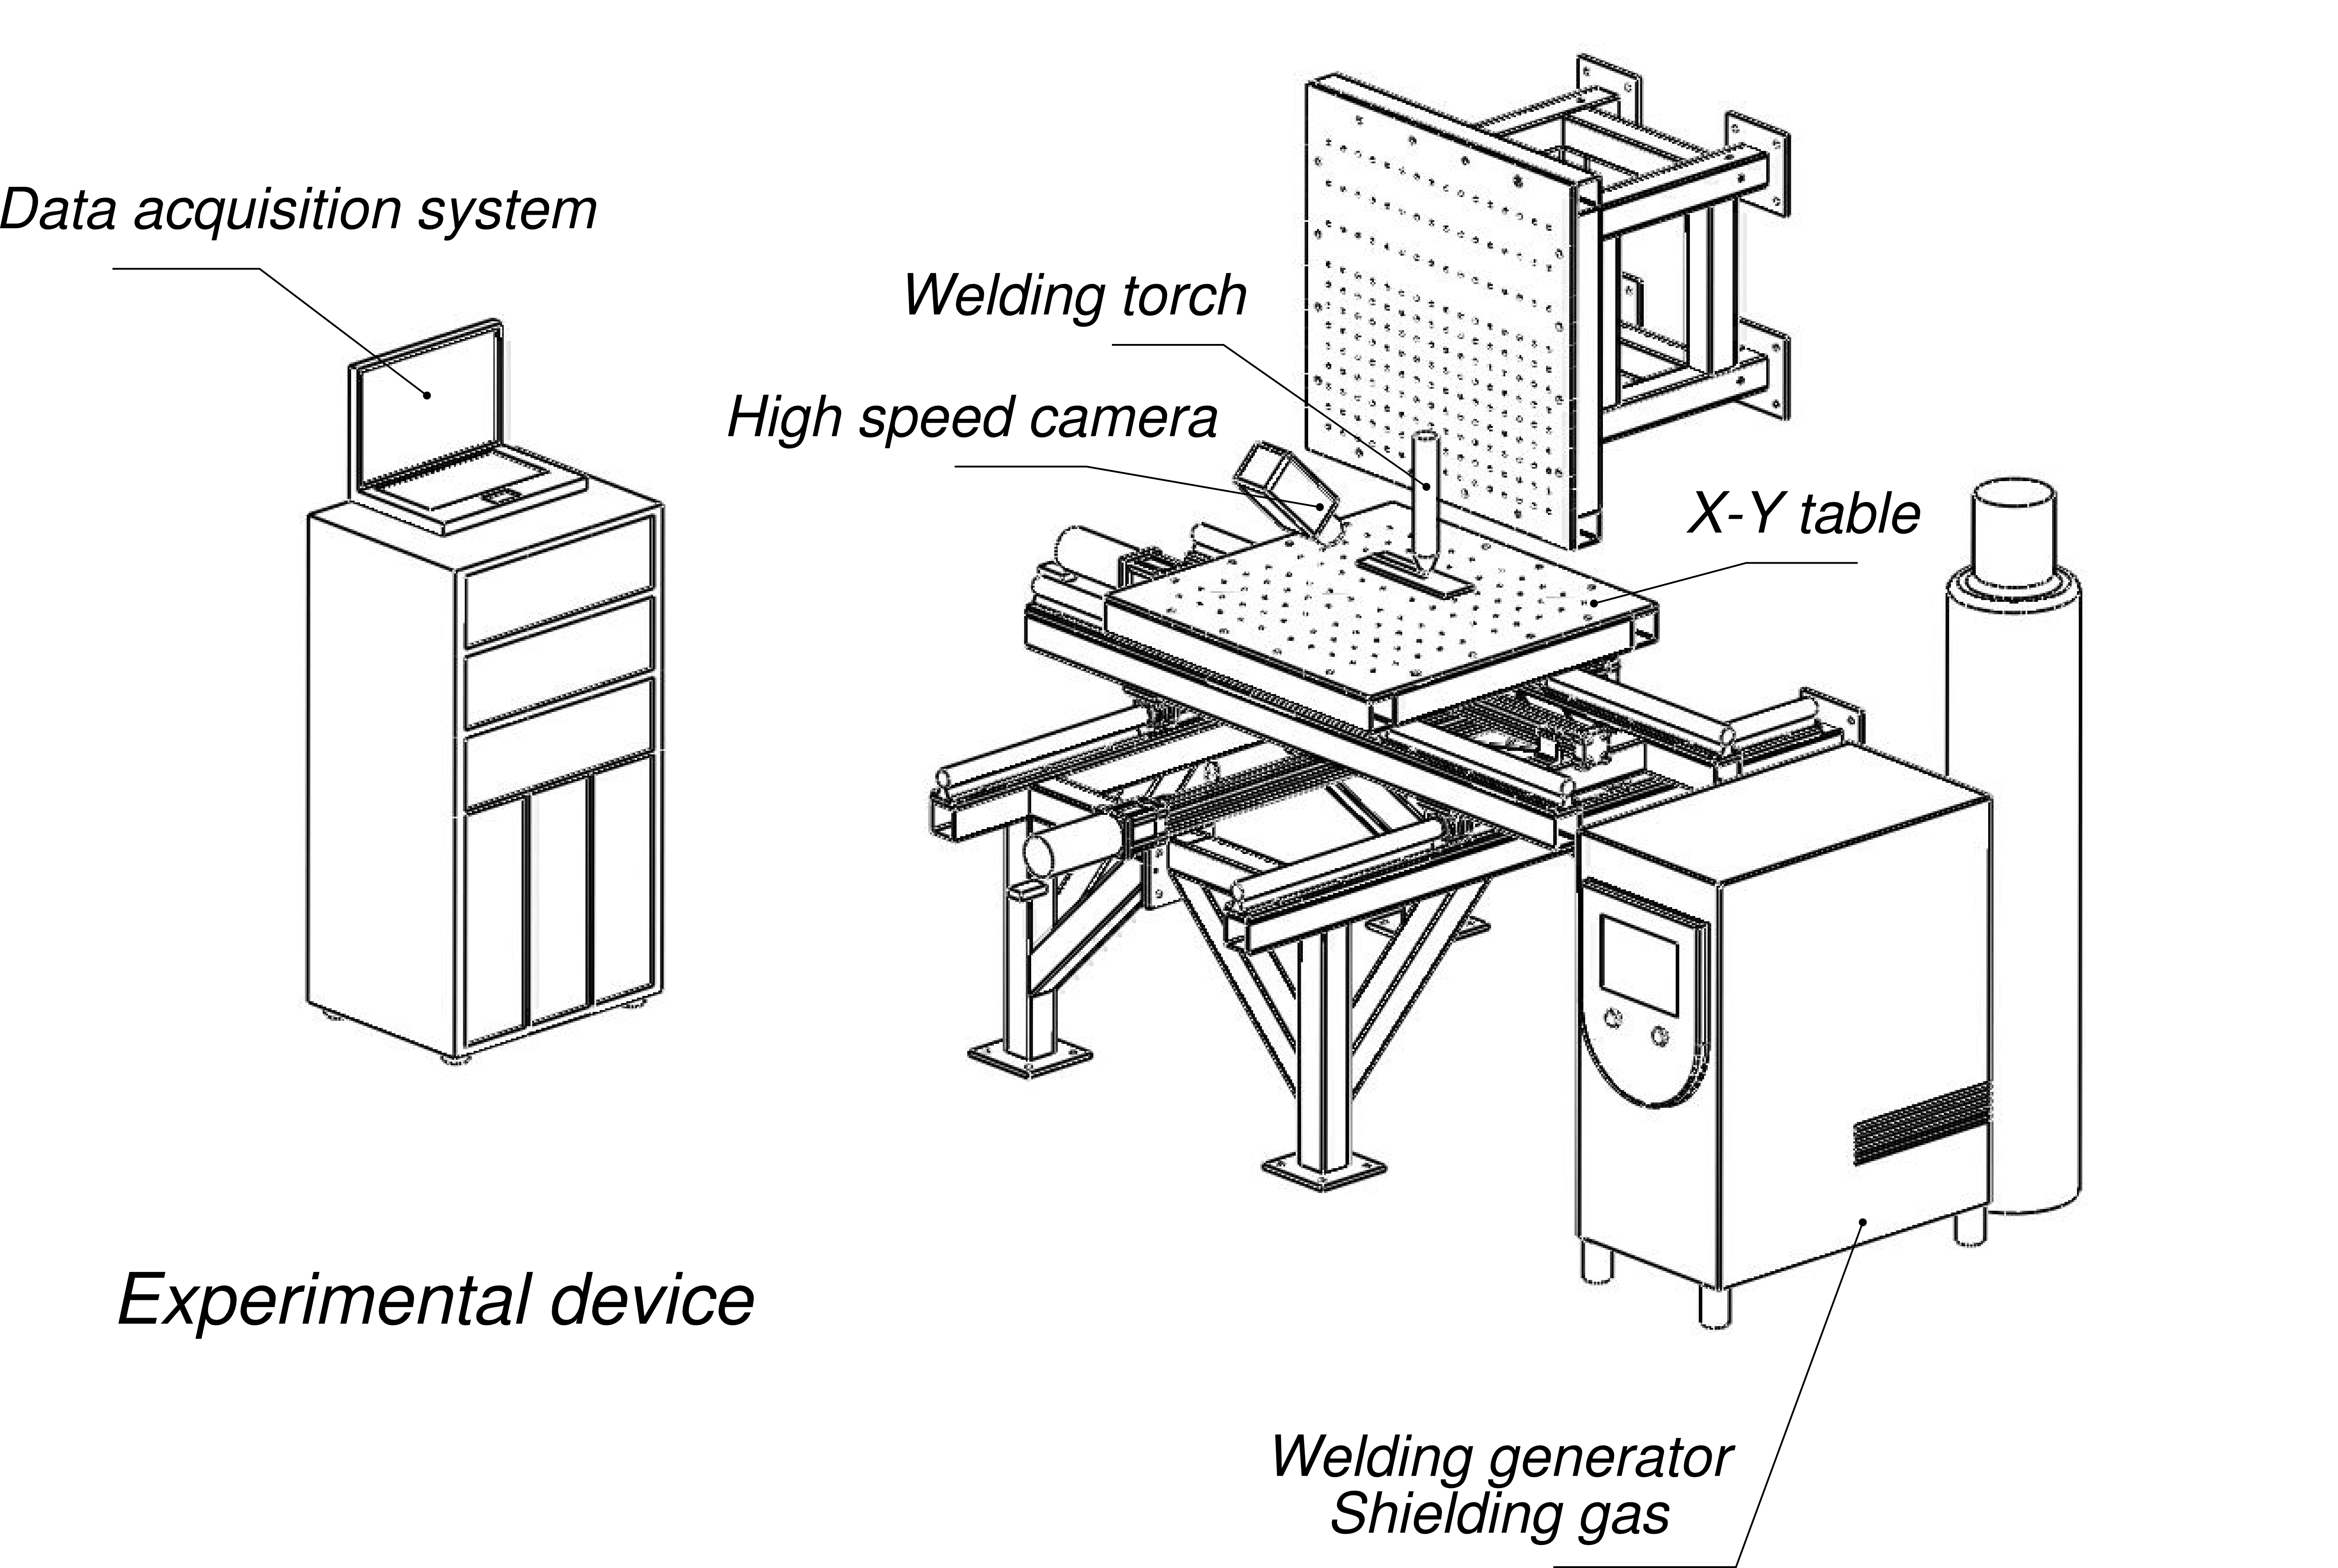
\includegraphics[width=7cm,height=4cm]{schema-platform.png}
\caption{{\small Experimental platform and specific device}}
\label{schema-platform}
\end{center}
\end{figure}

To compare and analyze the data two open source numerical libraries
 have been developed: The BAME (multi-physics measures data base)
 for all general data and the erCv specific to image treatment 
(including the spreading of welding pool geometry during welding).



\subsection{ Image acquisition setup}
\label{ image_acquisition_setup}

Using a similar technique employed by Kovacevic et al. \cite{KOVACEVIC}, the GTAW static process has been recorded by the specular reflection optical method. A $650\ nm$ laser diode has been used to light the weld process from an estimate angle of $35\ degree$. The laser beam width ($ $) was sufficient to guarantee a homogeneous illumination of the welding process. The laser projects an image by reflection of welding objects (weld pool and surrounding metal substrate) to the other side of the welding place. At this place and aligned with the optical path of reflected laser beam, a Phantom V5.0 high speed camera has been placed in order to record the process images (see figure \ref{schema-montage-experimental-GTAW}). 

\begin{figure}
\begin{center}
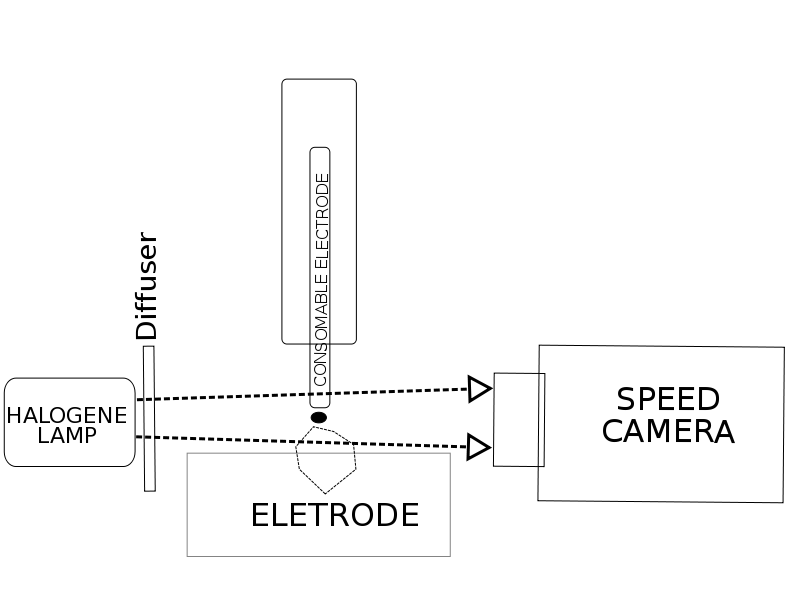
\includegraphics[width=7cm,height=4cm]{schema-montage-experimental-GMAW.png}
\caption{{\small Experimental setup to detect weld pool edges in GTAW process}}
\label{schema-montage-experimental-GTAW}
\end{center}
\end{figure}

To enhance the image contrast of the weld objects inside the electric discharge, the intensity rate between arc light and laser diode have to be reduce. In order to this a $650\ \pm 10\ nm$ band pass filter, which correspond to the laser diode wavelength, has been placed in front of the camera lens to attenuate the arc light. Nevertheless, the raw images remain highly noisy by the arc light. 


\subsection{ Welding condition}
\label{ welding_conditions}

Stationary spots weld are made using the GMAW process with the Oerlikon
 CitoWave 500 generator. The target is a steel disk of $10\ mm$ of
 thickness and ER70S steel welding wire.
The test campaign began by a reference test, with parameters fixed
 to:  welding time $4\ s$, wire feed speed $6\ m/min$, frequency 
droplets $113\ Hz$ and percentage of shielding gas ($CO_{2}$) $8$
 (so $92\%$ argon). Welding parameters values are summarize in 
tables \ref{table-parameters-static} to static and
 \ref{table-parameters-change} to variables parameters.

\begin{table}
\begin{center}
\begin{tabular}{|cc|}
\hline
Welding wire type & ER70S \\ 
Wire diameter ($mm$) or $drw$ & 1 \\  
Contact tip to work distance ($mm$) & 20 \\
Shielding gaz flowrate ($l/min$) & 18 \\ \hline
\end{tabular}
\caption{{\small Determined constant welding parameters used in experiments}}
\label{table-parameters-static}
\end{center}
\end{table}

\begin{table}
begin{center}
\begin{tabular}{|cc|}
\hline
Welding wire type & ER70S \\ 
Wire diameter ($mm$) or $drw$ & 1 \\  
Contact tip to work distance ($mm$) & 20 \\
Shielding gaz flowrate ($l/min$) & 18 \\ \hline
\end{tabular}
\caption{{\small Variable welding parameters used in experiments}}
\label{table-parameters-change}
\end{center}
\end{table}


Welding current and arc voltage are recorded at $30\ kHz$ 
sampling rate. The images are recorded at $4000$ frames per
 seconds, which is enough to measure macro drop radius and 
apparent liquid-solid contact angle histories. The images 
and electrical signals are synchronize, thanks to the 
automatically approach made in the multi physics platform.

Measurements are made using the erCv library.




\section{ System definitions}
\label{system_definitions}
\subsection{ Weld Pool}
\label{ weld_pool}

The purpose is to study the evolution of weld pool 
object in a GTAW process. Therefore it is necessary 
to detect the contour, without predetermined shape, 
of the weld pool and calculate his surface area. 

\begin{figure}
\begin{center}
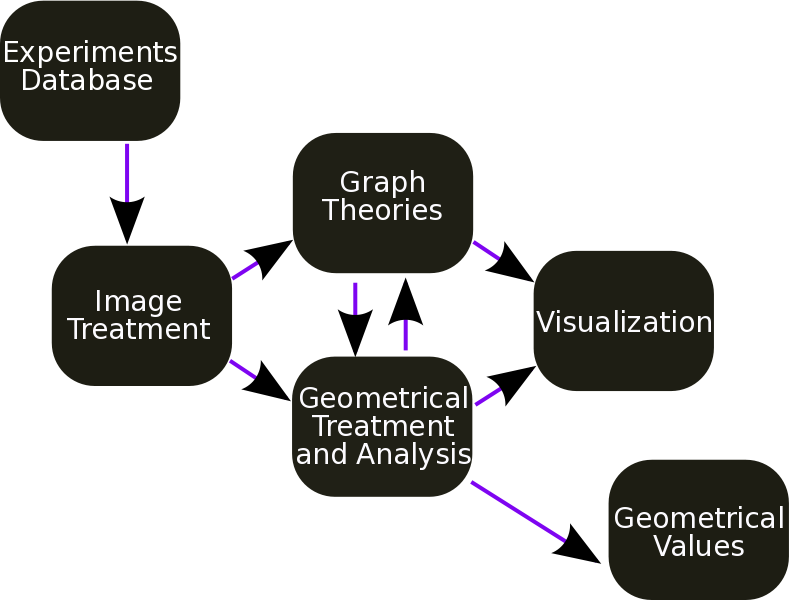
\includegraphics[width=7cm,height=4cm]{schema-erCv.png}
\caption{{\small Overview schematics of welding objects in a GTAW process}
\label{schema-macro-drop-droplet-parameters}
\end{center}
\end{figure}

At figure \ref{figure_1} appears the geometrical elements
 to be study at the weld pool: the weld pool contour and surface area.




\section{ The Analyze methods}
\label{ the-analyze-methods}

\subsection{ Image Calibration}
\label{ image_calibration}

As was shown in section \ref{image-acquisition-setup}, the 
camera recording a specular reflection of the welding process.
 Therefore the image of the welding objects is not orthogonal
 to the optical axes of the camera. In order to correct the 
image perspective, a control image (small chessboard image 
with known real dimensions) has been recorded at the weld 
pool place. A transformation matrix has been build between 
the control image (chessboard recorded image) and the original
 digital image. To calibrate the image dimension (in pixels) 
to the real objects dimension (in millimeters), a conversion
 scale has been applied with the real dimensions of chessboard 
control image $conv = 1\ mm/ 20\ pixels$. 

\begin{figure}[h!]
\begin{center}    
\subfigure[Chessboard control image]{\label{photo-calibration-cuadro-patron}\includegraphics[width=3.5cm,height=3.5cm]{photo-calibration-cuadro-patron.png}}
\subfigure[Chessboard original digital image]{\label{photo-calibration-cuadro-origin}\includegraphics[width=3.5cm,height=3.5cm]{photo-calibration-cuadro-origin.png}}\\
\subfigure[Raw recorded image]{\label{photo-calibration-image-origin}\includegraphics[width=3.5cm,height=3.5cm]{photo-calibration-image-origin.png}}
\subfigure[Perspective corrected image]{\label{photo-calibration-image-corrected}\includegraphics[width=3.5cm,height=3.5cm]{photo-calibration-image-corrected.png}}
\end{center}
\caption{{\small Perspective image correction samples}}
\label{photo-calibration}
\end{figure}



\subsection{ Image Treatment}
\label{ image_treatment}

The idea is to recognize the weld pool from the raw image and 
therefore calculate his 2D surface area. This requires the 
identification of a well define weld pool contour. Several
 approaches could be uses to obtain the weld pool contour, such
 as edge detection techniques \cite{WU2}, Hough transforms
 \cite{OLSON} or geometrical weld pool division \cite{KOVACEVIC}.
 Nevertheless the most common approach is the image segmentation
 \cite{WANG}. That means to split in two or more fields the image.
  The object, in this case the weld pool, would be colored in one
 color and the rest of the image in other color \cite{COCQUEREZ}.
 Thanks to the optical method acquisition (specular reflection) a
 natural way to segment the images, could be separate its between
 the roughness (non homogeneous lighting colored zone) and non 
roughness zone (see figures \ref{photo-macro-drop-original}). 
Into the lighting zone at the images, the mirror like surface 
of the weld pool reflect a uniform dark surface to the camera
 while the solid metal surface reflect a diffuse colored 
surface \cite{WU2}. This particularity in the color and in
 the light distribution (roughness) at the image could be 
interpreted as different textures zones \cite{MATERKA}, in
 the same the way as the eyes recognize the texture in the object
 surface and$/$or images.
The texture analysis method to perform image segmentation is an
 image processing technique widely uses in biomedicine, satellite 
recognition, industrial quality control and others fields requiring
 image processing. There exist different approaches to texture 
analysis, each one using their own image analysis methods:
\begin{description}
\item[Structural] Represent texture by well defined primitives,
 and a hierarchy of spatial arrangements of those primitives.
\item[Statistical] Represent the texture indirectly by the 
non-deterministic properties that govern the distributions 
and relationship between the grey levels of an images.
\item[Model based] Using fractal and stochastic models, 
attempt to interpret an image texture by use of, respectively,
 generative image model and stochastic model.
\item[Transform methods] Using Fourier and wavelet transforms, 
represent an image in a space whose co-ordinate system has an interpretation.
\end{description}

. Most of them required complex image analysis using
 hierarchy decomposition (structural), fractal or stochastic model
s (model based) and Fourier or wavelet transforms (transforms methods) 
 Di BLA BLA use this  has been thedescribe  where the shadows zones are the projection of the macro drop and droplet.
